\documentclass[utf8]{../IncArticle}
\graphicspath{{../}}
%\usepackage{color}
\usepackage{todonotes}
% \usepackage{lmodern}




% *** PDF, URL AND HYPERLINK PACKAGES ***
%
\usepackage{url}

\title{Интерактивная методика извлечения\todo[inline]{Первоначальный заголовок: Методика ПРИОБРЕТЕНИЯ знаний из текстовых документов, основанная на анализе ответов пользователя и полисистемы онтологий} знаний из текстовых документов, основанная на полисистеме онтологий}

\AddAuthor{Черкашин}{Е}{вгений}{А}{лександрович}{Институт динамики систем и теории управления СО РАН, Иркутск, ул. Лермонтова 134, 664033}
\AddAuthor{Черкашин}{А}{лександр}{К}{онстантинович}{Институт географии им. В.Б. Сочавы СО РАН, Иркутск, ул. Улан-Баторская 1, 664033}}
\AddAuthor{Бычков}{И}{горь}{В}{ячеславович}{Институт динамики систем и теории управления СО РАН, Иркутск, ул. Лермонтова 134, 664033}
\AddAuthor{Паскал}{К}{ристина}{К}{онстантиновна}{Национальный исследовательский Иркутский государственный технический университет, Иркутск, ул. Лермонтова 83, 664074}
\AddAuthor{Белых}{П}{олина}{В}{асильевна}{Институт динамики систем и теории управления СО РАН, Иркутск, ул. Лермонтова 134, 664033}
\setcounter{page}{1}
\date{}
\begin{document}

\begin{abstract}
%\boldmath


  В докладе представляется идея подхода к представлению и индукции
  логического слоя представления контента, например, содержимого
  сайтов, юридических документов и т.п. Этот слой порождается на
  основе анализа результатов редактирования содержимого (контента) ---
  как текстовой составляющей, так и его существующей логической
  структуры. Варианты интерпретации того или иного изменения
  содержимого (исправление ошибки/значения или формирование нового
  высказывания) уточняются в результате диалога с пользователем. На
  принятие решения также влияют результаты анализа поведения
  пользователя, например, выделяются повторяющиеся переходы между
  редактируемыми документами определенных классов.

  Теоретической основой методики является представление предметной
  области в виде полисистемы онтологий, т.е. многослойной структуры
  понятий и отношений, которые отображаются между слоями через
  интерпретацию. Полисистема онтологий, представленных в виде
  семантических сетей, позволяет организовать диалог с пользователем,
  упорядочивать и классифицировать факты о предметной области, а также
  получать новые интерпретации формируемых концептов.

  В качестве тестовой среды для разрабатываемых технологий выбрана
  автоматизация деятельности нотариальной конторы и документооборот
  административных, хозяйственных и научных подразделений бюджетного
  учреждения. Документы, используемые в этих видах деятельности,
  обладают одним важным свойством --- содержащаяся в них информация
  представляется как в неструктурируемом, так и в структурируемом
  виде.

\end{abstract}

\begin{abstract}[english]
  Here we have English abstract
\end{abstract}


\introduction{}
% no \IEEEPARstart

В 2001 году Т.-Б.Ли предложил план развития интернет"=технологий
(семантический веб), который направлен на реализацию сетевых сервисов
со значительным уровнем интеграции логического слоя представляемой
информации. Информация размечается семантически, а программные агенты,
используя эту информацию, производят ее обработку с целью решения
конкретных практических задач пользователя.

Одной из основных проблем семантического веба является тот факт, что
большинство пользователей решают свои практические задачи и не
заинтересованы повышении своей квалификации до уровня позволяющего
использовать эти технологии в полной мере. В такой ситуации
технологические аспекты семантического веба должны быть полностью
скрыты, а программное обеспечение должно "варить кашу из
топора". Необходимо разрабатывать программное обеспечения управления
содержимым сайтов и юридических документов как технологий приобретения
знаний, где пользователю предоставляется роль источника дополнительной
информации для интегрированного в систему механизма поддержки принятия
решений.

Идею подхода удобно излагать на примере юридических документов,
которые в большинстве случаев содержат сведения об отношениях между
физическими и юридическими лицами, а также другими элементами. Эти
сведения в исходной или преобразованной форме используются в других
документах. Поэтому имеет смысл для каждого документа извлекать и
хранить достаточно детально представленное логическое описание таких
сведений, которое преобразуется в текстовый документ при помощи
шаблонов. Вариант преобразования определяется отображаемым документом,
т.е. документ задает контекст представления логического слоя.

К настоящему времени технологии Семантического Веба (СВ) предоставляют
формальные механизмы представления указанных отношений при помощи
стандартных форматов и структур данных, а также несколько механизмов
их логической обработки. Логический слой представления информации в СВ
представляет собой граф, состоящий из концептов (понятий) и отношений
между ними. В частности в юридическом документе физические и
юридические лица находятся с этим документом в отношении
"часть--целое", а также в их более точных и содержательных вариантах.

В настоящее время большинство вариантов использования онтологических
моделей предметных областей сводятся к решению задачи уточнения
диапазона релевантных документов в процессе поиска. Автоматизация
извлечения онтологий из текстовых документов базируется на
сканировании хранилищ документов: содержимого текста документов и их
метаданных, анализ результатов сканирования. Наблюдение за поведением
людей в процессе подготовки различных документов приводит к
заключению, что содержательные части документов, которые и
представляются в логическом слое, как правило, находятся в тех местах
текста, где чаще всего пользователи производят изменения. Поэтому,
информационная система, автоматизирующая процессы подготовки
документов, должна отслеживать изменения, вводимые пользователем, во
времени и в пространстве версий. Версии порождаются копированием
документа или использование его в виде шаблона нового
документа. Подвергаться анализу должна вся совокупность
изменений. Предлагаемый подход позволяет сузить объем обрабатываемой
информации за счет фокусировки алгоритмов анализа данных вблизи
изменений. Границы изменений задаются, например, свойствами формата
представления текста документа (гипертекстовой разметкой) или
существующей логической структурой одной из его [документа] версий.

Элементы логического слоя (концепты, объекты и отношения между ними)
формируются в результате применения алгоритмов анализа данных и
интервьюирования пользователя. Среда, контекст, [приобретения знаний]
включает в себя:
\begin{itemize}
\item полисистему онтологий, совокупно описывающую предметные области,
  имеющие отношение к представлению документа как структуры данных,
  так и его содержательного смысла;
\item история изменения документа и его логического слоя;
\item список последних изменений в текущей транзакции (новой версии);
\item история действий пользователя в системе (пользователь, например,
  выполняет типичный набор действий по подготовке стандартного пакета документов);
\item ответы пользователя на утоняющие вопросы системы, цель которых
  --- определить [истинные намерения пользователя] смысл сделанных исправлений.
\end{itemize}

В результате анализа этих данных формируются новый набор троек вида
\texttt{<subject, relation, object>}, [представляющих новые данные
нового документа/версии, представленные в логическом
слое]. Накопленные логические слои документов необходимо периодически
также сканировать на выявление стойких функциональных зависимостей
между значениями объектов. В результате этого анализа, предлагается
совершенствовать формат представления данных слоя, например применяя
реляционные таблицы в качестве хранилищ. [Метод функциональных
зависимостей применяется наоборот (т.е. данные - анализ - структура)].

Сеть взаимодействующих программных систем, в которых реализованы перечисленные функции,
обладает многими свойствами социальной сети. Основными видами обработки
информации в такой сети являются ввод, хранение, фильтрация и
передача, т.е. интеграция данных, а не их агрегация с целью порождения
комплексных отчетов. Поэтому применения специальных методологий
проектирования программного обеспечения при разработке таких систем
(или подсистем приобретения знаний описываемого вида), например,
объектно-ориентированных технологий, не является значительным
преимуществом. Горазда важнее обеспечить возможность функционирования
программ на [дешевом хостинге] и создания каналов данных на основе
современных стандартных форматах данных.

Интересным свойством такой социальной сети, реализующей, фактически,
распределенный документооборот, является требования к организации
обмена данными между пользователями в процессе подготовки документов
преимущественно в режиме off-line. Современные информационные
технологии позволяют хранить данные логического слоя в разметке
электронных документов \ref{microformats,RDFa} и в виде QR-кодов,
сопровождающих печатные варианты документов.

\begin{itemize}
\item there are no predominant common task to be solved with all the agents (computer and human);
\item each agent solves its special task, so the agent API’s and supported data format must be strongly standardized;
\item human users of the social network do most of the aggregation tasks personally including subconscious joint processing of unstructured and semantic information.
\end{itemize}

In this paper, we continue the development of the approach to document and site content management and integration [-2-], where human users play a role of data sources in the process of semantic data markup formation of the document content.

As a testing ground, we have chosen document preparation automation of a Russian notary office. Most of all operations over documents can be expressed as textual and logical layer changes, for example, data of the logical layer are copied from one document to another; sometimes roles of individuals mentioned in the documents are alternated; database collects client data for further reuse (lookup), \emph{etc}.

\section{Logical Markup Procedure of the Document Content}

The RDF standard describes informational resources as triples <subject, relation, object> in a context. The set of triples forms a graph (network) of data and relations reflecting knowledge. It is convenient to divide graphs to subgraphs and construct their hierarchic complexes \cite{b4}, resulting a hierarchy of contexts. In a general case, a context affects the interpretation of its set of triples. For example, family name and passport data are presented as texts in different parts of the document, but related to the single person in the context defined by the document.

The rendering engine we considered in [-2-]. In this approach, all the template data for document rendering is also stored in the ontology graph. We also represent the views and algorithms implementing controllers in the sense of MVC (Model View Controller) technique with triples \cite{b5}. The content of the document from a general view is a tree, where almost each node is both a subject and an object of their corresponding relations (fig.1). The exceptions are the root node\,: it plays only the role of subject, and the leaf nodes that are objects only. In the higher level hierarchies, e.g. in a tree of the documents in a warehouse, the root node is an object node as well (it is referred from a record of the warehouse).

One of the key points of the research is semantic document markup techniques adaptation to the process of document editing. We suppose that a document body change, in a regular case, affects the meaning of the document, hence, alters its logical layer. Examples of the modifications are the elementary error correction, a field value change (an object of a triple), paragraph text editing that might imply its origin template correction. Each change also might result in a new triple relation construction between context subjects and old/new object value. The text change analysis is aimed at data and knowledge acquisition, where the content management system plays an active role, and user is a source of complementary information.

The semantic layer enrichment is carried on in an environment containing logic information thanks to document is already supplied with a logical layer. The source data for an acquisition step is as follows\,: a) the source version of the document, b) a text modification expressed in diff format \cite{b9}; c) user answers to the question asked by the system, which refine the semantics and structure of the modifications; d) user actions preceding the modification. If the modification corresponds to a value of an object of a triple then the modification means either error correction (subject is not changed) or creation of a new subject if user copied the document previously. Creation of a new document implies filling in a number of triples with new values representing a new subject (RDF resource) of the document.

If a field or a text is partially modified this can be interpreted as:
\begin{itemize}
\item again, an error correction without document meaning change;
\item a refinement of the logical structure of subject, extraction of a relation and an object; this corresponds to a new triple connecting the subject to the new object (changed value); the user must choose the subject of the new triple.
\end{itemize}

The new subject is chosen from a tree of all the subjects of the edited document. After the choice is made, a list of all available relation is constructed from all known relation of the subject, its class and parent classes. User must choose one relation to form the triple. In the case, when the list contains no desired relation, a new one must be defined. New relation is always a subclass of one that already exists in the system, which is also chosen from the list. New relations defined by inexperienced user must be periodically analyzed by knowledge engineers to get rid of semantic inaccuracy, contradictions, redundancy to the equivalents, and be, hence, refactored.

If a value of a triple is removed, then the triple is being removed too. The situation is acceptable if the minimal structural and semantic completeness of all the subjects of the documents are hold, otherwise either the user delete action is prohibited or the chain recursive deletion of the subjects is initiated. To control this behavior each subject class have to be accompanied with a list of minimal valuable triplets that define the basis of the subject meaning. Partial text removal, if it is not an error correction, is processed analogously to modification, with removed part being the object value. Addition of characters to text is an action similar to modification, i.e., in a general case a new triple is constructed.

Addition of a triple might result in extending the document with new subjects and relations. For example, let construct a new tripartite agreement from an existing bilateral one. In new contract a third individual appeared, so the addition of a new family name of the individual results in construction of a subject for the individual, filling in the necessary triples, as well as definition of a new relation between document and the subject as a subclass of structuralElement relation.

\section{Theoretical Generalization of the Acquisition Process}

The above described approach is a stepwise implementation of polysystem analysis and synthesis \cite{father} (PSAS) procedure. This is a general procedure for system analysis of domains. The essence of the approach is that domain and any its object or process can be fibrated and represent it in multidimensional space of fiber-coordinates. This approach is used in control problem solution, decomposition, analysis and synthesis of complex systems. In comparison to system approach, where the principle of interconnection of the elements is fundamental, polysystem analysis assumes the hypothesis of fibration, i.e., it supposes a possibility of representation of the object under investigation as disjoint subsets, thus, mutually unbound fibers (subdomains). So, in a generalized insight a polysystem is a system itself, and polysystem analysis is a new form of system analysis.

The application of the PSAS to the process of data and knowledge acquisition in the documents expressed as simultaneus polysystem fibering the domain in various coordinate systems (aspects) as follows\,: structural organization of a document (mereological aspect), expressing domain of activity area, hierarchical inheritance of various kind of documents (domain system concept inheritance), people and organization relationship, deontic logic representation of the document meaning, etc.

According to PSAS \cite{father} each concept of an aspect should be presented (via interpretation morphisms) in all other fibers as well as its relationships with adjacent concepts. Theoretically, for each of the fibers, a complete theory of the domain can be constructed. Each theory differ by their fundamental concept, but they are similar each other via concept substitution (an interpretation); this allows us to induce new axiomatic theories of domains in the image and likeness of the known ones. Each system domain (fiber) of knowledge fibrates multiply and sequentially, giving raise of the polysystem of representation of an object under investigation. All the system theories are combined in the unified model describing the domain and the object.

In our case we defined the procedure of triples acquisition as an instance of the fibration procedure. The obtained classes of documents, people and other objects are the concept of a PSAS theory of an aspect. Having established new class or new relation between two classes, the concept or relation should be reflected as a substituted (interpreted with) one in other ontologies (e.g., mereological one). In a general case we must also produce the definitions for the notions in those ontologies.

Each of new concept (a class) as we described in the previous section
is to be inherited from a parent class, thus, it can be interpreted in
other ontologies as either a concept that corresponds to the parent
class or to a new inherited class. This case the user interview also
organized to obtain a description of the class and the relation.

Thus, the usage of the PSAS allows us to partially deal with the
completeness (As \ldots{} \cite{sergey}) and consistency (by testing
an ontology and morphing the results to other ones) of the ontological
theories under construction.

\subsection{Utilizing Polysystem of Ontologies in User Interview}
As it was mentioned above any studied and modeled domain can be fibrated and represented as a polysystem of notions, objects and their relationships. The polysystem from a general point of view is a set of disjoint layers. Each layer contains a system of concepts, individual objects and corresponding relationships between them. In a fibrated polysystem, concepts belonging to a layer are morfed (mapped) into concepts in other layers via concept interpretation of one layer (projection, theory, science, domain) into concepts of other layer. All the concepts are interpreted by concepts of the abstract system layer. The interpretation feature of polysystem layers could be used to drive user interview dialog on the base of an inference by analogy represented as movement along relations and morphs in the polysystem of ontologies.

Consider simple family relationships in fig.~\ref{OPSA}, where most of the obvious relations are hidden to make the figure more readable. There are four main layers in the figure, which model corresponding aspects of Bob's family: layer 1 represents the family itself, it is the only layer having a-box entities; layer 2 represent main roles of individuals in a family; layer 3 shows genders as two opposites; and later 4 corresponds to mereological metomodel ``whole--parts''.

Let's construct a list of questions to determine a role of Jul in Bob's family. It is supposed we know only that Jul is a female. To put Jul in layer 1, we must ask a general question: ``Is Jul a part of Bob's family?'' The question is constructed according to a following intuitive inference. All relations between a family and its members are kinds of ``partOf:'' relation from layer 4. This fact is shown as an arrow, which denote a contravariant functor from category of Layer 2 to category of Layer 4, from relation hasFather: of Layer 2 to ``partOf:'' of Layer 4, other four arrows are hidden. So, in order to determine the fact that Jul is a member of Bob's family, it is sufficient to ask ``Is Jul partOf: Bob's-family?''. The identifier of the example family is devised from the tradition to name families after their master of housekeeping (MOH) person, that is denoted by arrow from individual Bob (layer 1) to concept MOH (layer 2).

If user answered positively (Jul is a part of the family), then we must refine her role, as partOf: is not a role allowed to be used in layer 1. Jul is a female (by definition), so she cannot be father and son. If she is, she must be male, but it is not as male and female are formally opposite concepts. If multiplicity of relations in the layer are defined, then we will also know, that the family already has mother. The only possible choice is Jul is daughter, resulting an another general question:''Is Jul daughter?'' If the answer to the second question is also positive, finally a new triple constructed <Bob's-family hasDaughter: Jul>.

If, e.g., gender of Jul is unknown, then the second question is constructed as a special question ``What role has Jul in Bob's family?'' and a list of two possible answers is shown: ``hasDaughter:'' and ``hasSon:''. Or it can be constructed as an alternative question ``Is Jul plays hasDaughter: or hasSon: role in the family?'', but in this case the sentence is more weird with respect to English.

\begin{figure}
\centering\sf
\def\svgwidth{0.9\linewidth}
\input{layer.pdf_tex}
\caption{An  Usage Example of an Ontology Polysystem}
\label{OPSA}
\end{figure}



(HERE: a generalizing resume paragraph needed.)

(About polysystem of ontologies).

(procedure of fibration)

(procedure of completeness reconstruction): (About mapping via functors).

(Induction of notions, suppositions of fibrations).

(wikipedia and Google search systems).

(!! Systems of complexes. !!)

\section{An Office Usage of the Technique}

One of the applications of the technology under development is document preparation automation of a notary office. Notary office in Russia generate vast amount of printed documents. The documents contain both formalized and unformalized data in a balance reasonable for our study. For example, formalized data are the passport data of individuals, registration data of vehicles. Data of this kind are passed from one document to other documents mostly sturcturized and unchanged, raising a bindles of related documents. The document content structure significantly depends on entry fields’ data filled in: form of notary signature field depends on legal capacities of the individuals mentioned in the main document body. At present templates of the documents are prepared by a programming engineer collaborating with a professional secretary and verified by supervising notary. Unformalized data are various enumerations of legal empowerments of the individuals, article codes, and explanatory text.

Application of the semantic approach to the logical layer representation of the notary document content is aimed at involvement of the secretaries (people with low engineering skills) into the processes of the document instances preparation from the existing templates and into the development of the templates and constructing their hierarchical arrangement.

Logical layer of a notary document consists of hierarchy of subjects. The subjects relate to each other on various abstraction levels, e.g., in a letter of attorney there are at least two individuals, the first one is principal, and the second one is trusted (proxy). For each individual passport, data and place of residence are defined. The letter can contain other person data, e.g., for partially capable children. All the individuals are in explicit relation to the document. The triples <letatt998 containsPrincipal indiv\_78> and <letatt998 containsProxy indiv\_79> could define a principal and proxy to the document. The mentioned relations are specifications of abstract hasIndividual and structuralElement relations. This multilevel approach allows us visually represent hierarchical structures of the document, having interpreted the relations as structural elements, and in the same time to associate individuals with other roles in new documents, swap roles during editing. The swap function is implemented as user interface widget, which recognizes certain subject-to-subject relation patterns in the document body and interprets semantics of the relations as possible action. A general graph structure of the abstract level of a notary office automation ontology is drawn in fig.~\ref{notaryontology}.

[The flexibility and minimum resources and administration requirements criteria are of very importance to choosing database providing information resources storage as triples. The database management systems as DB2, Oracle and SQL Server cannot fulfill requirements because after running the operation is performed as a separate process. Also application and DBMS interaction should be implemented through interprocess communication form.

Solution to these problems is achieved by using the built-in database management systems that provide communication with the application at the same level of address space. This allows the application based on the built-in database to be efficient and autonomous.

Kyoto Cabinet is a library of routines for managing a database. The database is a simple data file containing records, each is a pair of a key and a value. Every key and value is serial bytes with variable length. Both binary data and character string can be used as a key and a value. Each key must be unique within a database. There is neither concept of data tables nor data types. Records are organized in hash table or B+ tree. \cite{b1}

Availability of funds to work with triplets described in the standard RDF is an advantage database management system Kyoto Cabinet over other embedded systems is. In this case the developer does not need to spend time on design and implementation of the data model so that its performance on this task is increased.

1.	Kyoto Cabinet. URL: http://fallabs.com/kyotocabinet/ (дата обращения: 20.02.2014).]



%\subsubsection{Subsubsection Heading Here}
%Subsubsection text here.




% An example of a floating figure using the graphicx package.
% Note that \label must occur AFTER (or within) \caption.
% For figures, \caption should occur after the \includegraphics.
% Note that IEEEtran v1.7 and later has special internal code that
% is designed to preserve the operation of \label within \caption
% even when the captionsoff option is in effect. However, because
% of issues like this, it may be the safest practice to put all your
% \label just after \caption rather than within \caption{}.
%
% Reminder: the "draftcls" or "draftclsnofoot", not "draft", class
% option should be used if it is desired that the figures are to be
% displayed while in draft mode.
%
\begin{figure}[!t]
\centering
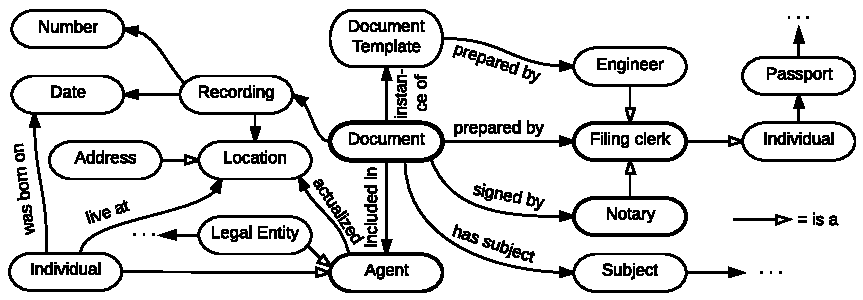
\includegraphics[width=\linewidth]{DocumentOntology-en.pdf}
% where an .eps filename suffix will be assumed under latex,
% and a .pdf suffix will be assumed for pdflatex; or what has been declared
% via \DeclareGraphicsExtensions.
\caption{An upper layer of notary office ontology}
\label{notaryontology}
\end{figure}

% Note that IEEE typically puts floats only at the top, even when this
% results in a large percentage of a column being occupied by floats.


% An example of a double column floating figure using two subfigures.
% (The subfig.sty package must be loaded for this to work.)
% The subfigure \label commands are set within each subfloat command, the
% \label for the overall figure must come after \caption.
% \hfil must be used as a separator to get equal spacing.
% The subfigure.sty package works much the same way, except \subfigure is
% used instead of \subfloat.
%
%\begin{figure*}[!t]
%\centerline{\subfloat[Case I]\includegraphics[width=2.5in]{subfigcase1}%
%\label{fig_first_case}}
%\hfil
%\subfloat[Case II]{\includegraphics[width=2.5in]{subfigcase2}%
%\label{fig_second_case}}}
%\caption{Simulation results}
%\label{fig_sim}
%\end{figure*}
%
% Note that often IEEE papers with subfigures do not employ subfigure
% captions (using the optional argument to \subfloat), but instead will
% reference/describe all of them (a), (b), etc., within the main caption.


% An example of a floating table. Note that, for IEEE style tables, the
% \caption command should come BEFORE the table. Table text will default to
% \footnotesize as IEEE normally uses this smaller font for tables.
% The \label must come after \caption as always.
%
%\begin{table}[!t]
%% increase table row spacing, adjust to taste
%\renewcommand{\arraystretch}{1.3}
% if using array.sty, it might be a good idea to tweak the value of
% \extrarowheight as needed to properly center the text within the cells
%\caption{An Example of a Table}
%\label{table_example}
%\centering
%% Some packages, such as MDW tools, offer better commands for making tables
%% than the plain LaTeX2e tabular which is used here.
%\begin{tabular}{|c||c|}
%\hline
%One & Two\\
%\hline
%Three & Four\\
%\hline
%\end{tabular}
%\end{table}


% Note that IEEE does not put floats in the very first column - or typically
% anywhere on the first page for that matter. Also, in-text middle ("here")
% positioning is not used. Most IEEE journals/conferences use top floats
% exclusively. Note that, LaTeX2e, unlike IEEE journals/conferences, places
% footnotes above bottom floats. This can be corrected via the \fnbelowfloat
% command of the stfloats package.



\conclusion
An approach to representation of logical layer of a document based on RDF (Resource Description Framework) is proposed. The approach allows us to formalize the structure and semantic relation of the document, and also store data to render the document as HTML-page in the same data format - RDF. XML and RDF allow us to join logical and presentation aspects of the document within the same storage engine. The engine stores data as an onology, i.e., set of triples <subject, relation, object>. A technique for HTML-rendering from the logical layer is described. The resulting document will contain the logical layer as a RDFa markup. The generated RDFa-markup is used at client side by web-browser for control of WYSIWYG-editing of the document. Text elements are modified with special widgets appearing in the user interface on an mouse event. A technique for organization of an interactive process of logical layer forming of the document content on the base of modifications analysis of the document content introduced by user. An example of application of the technologies under development in a notary office is presented. Thus, we shown that RDF format mixed with XML allows us to represent logical layer of meaningful information of a document, as well as sharing common data between documents.

On the base of the technology a network of document data exchange can be devised. The security of the document transmission can be provided as off-line data streams: each physical document is accompanied with its bar- or QR-code encoding the corresponding RDF-data of the transferred document. This can result in a semantic network analogous to nowadays social networks.

A part of the paper devoted to consideration of organizational problems, such as involving knowledge engineers in a refinement process of generated parts of the ontologies; partial automatic ontology verification; implementing secure ways of personal data transfer and processing. The properties of the document exchange network will be similar to social networks, and, probably, can be further developed and investigated the same way.



% conference papers do not normally have an appendix


% use section* for acknowledgement
\thanks
The research is carried on under support of Integration multidisciplinary project of Siberian Branch of Russian Academy of Sciences N 17 “Development of services and infrastructure of scientific spatial data for supporting complex multidisciplinary scientific research of Baikal nature territory”.

%The authors would like to thank...





% trigger a \newpage just before the given reference
% number - used to balance the columns on the last page
% adjust value as needed - may need to be readjusted if
% the document is modified later
%\IEEEtriggeratref{8}
% The "triggered" command can be changed if desired:
%\IEEEtriggercmd{\enlargethispage{-5in}}

% references section

% can use a bibliography generated by BibTeX as a .bbl file
% BibTeX documentation can be easily obtained at:
% http://www.ctan.org/tex-archive/biblio/bibtex/contrib/doc/
% The IEEEtran BibTeX style support page is at:
% http://www.michaelshell.org/tex/ieeetran/bibtex/
%\bibliographystyle{IEEEtran}
% argument is your BibTeX string definitions and bibliography database(s)
%\bibliography{IEEEabrv,../bib/paper}
%
% <OR> manually copy in the resultant .bbl file
% set second argument of \begin to the number of references
% (used to reserve space for the reference number labels box)
\begin{thebibliography}{11}

\bibitem{IEEEhowto:kopka}
H.~Kopka and P.~W. Daly, \emph{A Guide to \LaTeX}, 3rd~ed.\hskip 1em plus
  0.5em minus 0.4em\relax Harlow, England: Addison-Wesley, 1999.

\bibitem{TBL2001} T. Berners-Lee, J. Hendler and O. Lissila. \emph{The Semantic Web A new form of Web content that is meaningful to computers will unleash a revolution of new possibilities.}\hskip 1em plus 0.5em minus 0.4em\relax  Scientific American, May 17, 2001, pp.1-18. URL: http://sciam.com/article.cfm?articleID=00048144-10D2-1C70-84A9809EC588EF21. (access date: 05.09.2013).
\bibitem{q1}
Social network - Wikipedia, the free encyclopedia. URL: \url{http://en.wikipedia.org/wiki/Social_network} (access date: 20.08.2013).
\bibitem{q2}
Chameleon – Chameleon 2.10 documentation. \url{http://chameleon.readthedocs.org/en/latest/} (access date:  20.08.2013).
\bibitem{q3}
Virtuoso Open-Source Edition URL: \url{http://virtuoso.openlinksw.com/dataspace/doc/dav/wiki/Main/} (access date: 30.05.2013).
\bibitem{q4}
PIZZA Protege OWL tutorial at Manchester (School of Computer Science - The University of Manchester)  URL:\url{http://owl.cs.manchester.ac.uk/tutorials/protegeowltutorial/} (access date: 20.09.2013).
\bibitem{q5}
SWI-Prolog's home. URL: \url{http://www.swi-prolog.org/} (access date: 20.08.2013).
\bibitem{q6}
The Protégé Ontology Editor and Knowledge Acquisition System. URL: \url{http://protege.stanford.edu/} (access date: 20.08.2013).
Semantic MediaWiki. URL: \url{http://semantic-mediawiki.org/} (access date: 20.08.2013).
\bibitem{q7}
N.Heino, S.Tramp, N.Heino, S.Auer. Managing Web Content using Linked Data Principles – Combining semantic structure with dynamic content syndication. Computer Software and Applications Conference (COMPSAC), 2011 IEEE 35th Annual. pp. 245 - 250. URL:\url{http://svn.aksw.org/papers/2011/COMPSAC_lod2.eu/public.pdf} (access date: 30.05.2013).
\bibitem{q8}
Cherkashin E.A., Paramonov V.V., et al, Model Driven Architecture is a Complex System, E-Society Journal Research and Applications. Volume 2, Number 2, 2011, pp. 15-23.
\bibitem{q9}
Father


\end{thebibliography}

% that's all folks
\end{document}

%% Local Variables:
%% eval: (ispell-change-dictionary "ru_RU_hunspell")
%% TeX-master: t
%% TeX-PDF-mode: 1
%% TeX-source-correlate-mode: 1
%% TeX-source-correlate-start-server: nil
%% End:
